% !TEX program = xelatex
\documentclass[aspectratio=169,9pt,handout]{beamer}
\usetheme{Compostela}
\usepackage{amsmath,amsfonts,amssymb,bm}

\definecolor{amber}{rgb}{1.0, 0.75, 0.0}
\definecolor{silver}{rgb}{0.75, 0.75, 0.75}

%\usepackage{pgfpages}
%\setbeameroption{show notes on second screen}

\usepackage{pdfcomment}
\newcommand{\pdfnote}[1]{\marginnote{\pdfcomment[icon=note]{#1}}}
% \newcommand{\pdfnote}[1]{}


%%%%%%%%%%%%%%%%%%%%%%%%%%%%%%%%%%%%%%%%%%%%%%%%%%%%%%%%%%%%%%%%%%%%%%%%%%%%%%%%
%%%%%%%%%%%%%%%%%%%%%%%%%%%% Talk Configuration %%%%%%%%%%%%%%%%%%%%%%%%%%%%%%%%

\newcommand{\TalkPlace}{5th Red LHC Workshop}
\newcommand{\TalkAuthor}{
\href{mailto:marcos.romero.lamas@cern.ch}{Marcos Romero Lamas}
}
\newcommand{\TalkAuthorShort}{Marcos Romero}
% TODO: put this title in bold
\newcommand{\TalkTitle}{Latest LHC$b$ results on $\phi_s$}
\newcommand{\TalkTitleShort}{Latest LHC$b$ results on $\phi_s$}
\newcommand{\TalkInstitute}{}
\newcommand{\TalkDate}{May 10th}
\newcommand{\TalkDateNumber}{2021/05/10}

%%%%%%%%%%%%%%%%%%%%%%%%%%%%%%%%%%%%%%%%%%%%%%%%%%%%%%%%%%%%%%%%%%%%%%%%%%%%%%%%

\usepackage{adjustbox,multicol}

\usepackage{tikz,shapepar,booktabs}
\newcommand{\myparshape}{
{20}
{0}b{20}\\ 
{0}t{7.5}{20}\\ % corta arriba
{20}t{0}{30}\\  % corta abaixo
{20}e{10}
}

\usepackage{lipsum}

\usepackage{array}
\newcommand{\TupleVersion}{v0r5}
\newcommand{\FIGS}{/home3/marcos.romero/phis-scq/output/figures}
\newcommand{\PARS}{/home3/marcos.romero/phis-scq/output/tables}

\newenvironment{variableblock}[3]{%
  \setbeamercolor{block body}{#2}
  \setbeamercolor{block title}{#3}
  \begin{block}{#1}}{\end{block}}

%%%%%%%%%%%%%%%%%%%%%%%%%%%%%%%%%%%%%%%%%%%%%%%%%%%%%%%%%%%%%%%%%%%%%%%%%%%%%%%
\begin{document} %%%%%%%%%%%%%%%%%%%%%%%%%%%%%%%%%%%%%%%%%%%%%%%%%%%%%%%%%%%%%%
%%%%%%%%%%%%%%%%%%%%%%%%%%%%%%%%%%%%%%%%%%%%%%%%%%%%%%%%%%%%%%%%%%%%%%%%%%%%%%%



%%%%%%%%%%%%%%%%%%%%%%%%%%%%%%%%%%%%%%%%%%%%%%%%%%%%%%%%%%%%%%%%%%%%%%%%%%%%%%%
%%%%%%%%%%%%%%%%%%%%%%%%%%%% TITLE PAGE & CONTENTS %%%%%%%%%%%%%%%%%%%%%%%%%%%%
%%%%%%%%%%%%%%%%%%%%%%%%%%%%%%%%%%%%%%%%%%%%%%%%%%%%%%%%%%%%%%%%%%%%%%%%%%%%%%%

\begin{frame}[plain,overlaytitlepage=0.9,backgroundpicture=gpx/aiandes.pdf]
  \begin{minipage}[b][\textheight][b]{5cm}
    \includegraphics[height=0.5cm]{logos/igfae_bw}\hspace{1mm}
    \includegraphics[height=0.5cm]{logos/usc_bw}\hspace{1mm}
    \includegraphics[height=0.5cm]{logos/xunta_bw}\hspace{1mm}\\[2mm]
    \includegraphics[height=0.5cm]{logos/maeztu_bw}\hspace{1mm}
    \includegraphics[height=0.5cm]{logos/lhcb_bw}\\[-1mm]
  \end{minipage}
\end{frame}

\begin{frame}[plain,backgroundpicture=gpx/aiandes.pdf,overlaytoc=0.9]
  \addtocounter{framenumber}{-1}
  \hspace*{8cm}\begin{minipage}{8cm}
    \tableofcontents
  \end{minipage}
\end{frame}

%%%%%%%%%%%%%%%%%%%%%%%%%%%%%%%%%%%%%%%%%%%%%%%%%%%%%%%%%%%%%%%%%%%%%%%%%%%%%%%



\section{Overview}

\subsection*{Why is \texorpdfstring{$\phi_s$}{phis} important?}

\begin{frame}[default,t]
  \frametitle{noframetitle}
  \begin{columns}
  \begin{column}{0.6\textwidth}
  \begin{itemize}
    \item $\phi_s$ is very sensitive to BSM physics.
    \item $\phi_s$ is the mixing-induced CPV phase in $B_s$ decays.
    $$ \phi_s = -2 \beta_s = -2 \text{arg} \left(-
    \frac{V_{ts}V_{tb}^*}{V_{cs}V_{cb}^*} \right) $$
    \item Assuming only SM tree level contribution:
  \end{itemize}
  \end{column}
  \begin{column}{0.3\textwidth}
    \includegraphics[width=0.75\textwidth]{gpx/phis_scheme.pdf}
    \vspace*{-20mm}$$\lambda_f = {\color{scqred}\frac{q}{p}}
    {\color{scqgreen}\frac{\overline{A}}{A}} \,\qquad \quad\,$$
  \end{column}
  \end{columns}

\bigskip

\begin{center}
\onslide<1>{\begin{tabular}{cccccc}
  $\phi_s^{SM} = - \text{arg}(\lambda_f) =$ &
  $\phi_M^{SM}$ &
  $-$ & 
  $ 2 \phi_{D} $ \\ 
    & \\
  &
  \includegraphics[scale=0.2]{gpx/bs_mixing.pdf} & & 
  \includegraphics[scale=0.2]{gpx/bs_decay_tree.pdf}
\end{tabular}}
\end{center}

\pdfnote{Fist things first, why do we care about phis?. Phis is a very sensitive
probe to BSM physics, and it appears in Bs decays. It is the mixing induce CPV
phase of those decays. It its very well predicted in the SM to be very small,
and equal to minus two betas, about 30 mrad.}
\pdfnote{Assuming only tree level in SM, it will be composed of the mixing phase
and the decay phase, as we see it here. But,}

\end{frame}



\addtocounter{framenumber}{-1}
\begin{frame}[default,t]
  \frametitle{noframetitle}
  \begin{columns}
  \begin{column}{0.6\textwidth}
  \begin{itemize}
    \item $\phi_s$ is very sensitive to BSM physics.
    \item $\phi_s$ is the mixing-induced CPV phase in $B_s$ decays.
    $$ \phi_s = -2 \beta_s = -2 \text{arg} \left(-
    \frac{V_{ts}V_{tb}^*}{V_{cs}V_{cb}^*} \right) $$
    \item NP could enter in $B_s^0$ mixing:
  \end{itemize}
  \end{column}
  \begin{column}{0.3\textwidth}
    \includegraphics[width=0.75\textwidth]{gpx/phis_scheme.pdf}
    \vspace*{-20mm}$$\lambda_f = {\color{scqred}\frac{q}{p}}
    {\color{scqgreen}\frac{\overline{A}}{A}} \,\qquad \quad\,$$
  \end{column}
  \end{columns}

\bigskip

\begin{center}
{\begin{tabular}{cccccc}
  $\phi_s = - \text{arg}(\lambda_f) =$ &
  $\phi_M^{SM}$ &
  $+$ & 
  $\Delta\phi_{NP}$ &
  $-$ & 
  $ 2 \phi_{D} $ \\ 
  & \\
  &
  \includegraphics[scale=0.2]{gpx/bs_mixing.pdf} & & 
  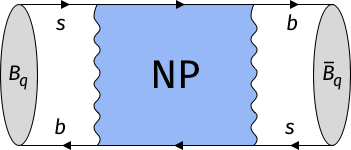
\includegraphics[scale=0.2]{gpx/bs_mixing_np.pdf} & &
  \includegraphics[scale=0.2]{gpx/bs_decay_tree.pdf}
\end{tabular}}
\end{center}


\pdfnote{New physics could appear in the Bs mixing. Thus, any deviation we see
of phis from the SM prediction could be a signature of BSM physics.}
\end{frame}



\subsection*{\texorpdfstring{$B_s^0 \rightarrow J/\psi K^+ K^-$}{Bs0toJpsiKK}
and \texorpdfstring{$B_s^0 \rightarrow J/\psi \pi^+ \pi^-$}{Bs0toJpsipipi}
channels}



\begin{frame}[default]
\frametitle{noframetitle}

\begin{columns}[T]
  \begin{column}{0.55\paperwidth}
  \begin{itemize}
    \item $\phi_s$ is most precisely measured in $b \rightarrow c \bar{c} s$
    processes. Where (SM) penguin pollution is small.
    \item $B_s^0$ decays are an addmixture of CP-even and CP-odd final states.
    \item Higher order penguin contributions can also appear in $\phi_s$.
    \begin{itemize}
      \item Need to control penguin pollution $\phi_s = -2\beta_s
      + \Delta\phi_s^{\text{peng}} + \Delta \phi_s ^{NP}$.
      \item For $B_s^0 \rightarrow J/\psi \phi$, $SU(3)$ counterparts where $T
      \sim P$  ($B_s^0 \rightarrow J/\psi \{\rho, K^{*0}\}$) are used to
      estimate penguin contributions.
    \end{itemize}
  \end{itemize}
  \end{column}

  \begin{column}{0.35\paperwidth}
    \vspace*{-10mm}
    \begin{variableblock}{Golden mode: $B_s^0 \rightarrow J/\psi K^+ K^-$}
    {bg=amber!20}{bg=amber}
      \begin{itemize}
        \item Relatively large BF of $\mathcal{O}(10^{-3})$
        \item Measurement of $\Gamma_s = \frac{\Gamma_H+\Gamma_L}{2}$, 
        $\Delta \Gamma = \Gamma_L - \Gamma_H$ and $\Delta m_s = m_H - m_L$.
      \end{itemize}
    \end{variableblock}

    \begin{variableblock}{Silver mode: $B_s^0 \rightarrow J/\psi \pi^+ \pi^-$}
    {bg=silver!20}{bg=silver}
      \begin{itemize}
        \item BF of $\mathcal{O}(10^{-4})$
        \item Crosscheck of $B_s^0 \rightarrow J/\psi K^+ K^-$
        \item CP-odd (mainly), direct access to $\Gamma_H$
      \end{itemize}
    \end{variableblock}
  \end{column}
\end{columns}

\begin{center}
  \includegraphics[width=0.85\textwidth]{gpx/topologies.pdf}
\end{center}

\pdfnote{Phis is most precisely measured in b to c c s transitions. Here the SM
penguin is predicted to be small. Generally Bs decays are an addmixture of CP
event and CP idd states we need to disentangle in order to get phis.}
\pdfnote{However, in order to claim NP, we nee to have the penguing pollution
really well under control. Otherwise we could be confusing NP with penguin
contricontributions. That's why we use control channels JpsiRho and JpsiKstar to
estimate penguin contributions there, were they are not supressed wrt tree
level.}
\pdfnote{Finally, the two main channels to measure phis are Bs2JpsiKK(Phi), and
Bs2JpsiPiPi...}

\end{frame}



\subsection*{Ingredients} % {{{

\begin{frame}[default] 
\frametitle{noframetitle}

\begin{columns}%[T]
  \begin{column}{0.45\textwidth}
    \begin{variableblock}{Time-dependent asymmetry in the SM}{bg=scqblue!20}{bg=scqblue}
      \centering $\mathcal{A}_{\text{CP}} = \frac{\Gamma[\overline{B}{}_s^0 \rightarrow f] - \Gamma[{B}{}_s^0 \rightarrow f]}{\Gamma[\overline{B}{}_s^0 \rightarrow f] + \Gamma[{B}{}_s^0 \rightarrow f]} \approx \eta \sin \phi_s \sin \Delta m_s t $
    \end{variableblock}
    \tiny \hspace*{-5mm}
    \[p.d.f. = \frac{\displaystyle
      \sum_{u,v={S,0,\parallel,\perp}} \!\!\!  
        C_{u,v} 
        \,\,\, 
        A_{u} \overline{A}_{v}
        \,\,\, 
        f_{u,v} [\Omega]
        \,\,\,  \left\{  
        h_{u,v}^{B_s^0}[t] +  
        h_{u,v}^{\overline{B}_0^s}[t]  \right\}
      }{\displaystyle \int_{0.3 \, \text{ps}}^{15 \, \text{ps}}dt \int_{\Omega} d\Omega
      \sum_{u,v={S,0,\parallel,\perp}} \!\!\!  
        \,\,\, 
        A_{u} \overline{A}_{v}
        \,\,\, 
        f_{u,v} [\Omega]
        \,\,\,  \left\{  
        h_{u,v}^{B_s^0}[t] +  
        h_{u,v}^{\overline{B}_0^s}[t]  \right\} 
      }\]
    
      \begin{center}
        \includegraphics[width=0.6\textwidth]{gpx/HelicityPlanes}
      \end{center}
  \end{column}

  \begin{column}{0.45\textwidth}
    \begin{variableblock}{We experimentally measure }{bg=scqorange!20}{bg=scqorange}
      \centering $\mathcal{A}_{\text{CP}} \approx  (1-2\omega) e^{-\frac{1}{2} {\Delta m_s}^2 {\sigma_t}^2 } \eta \sin \phi_s \sin \Delta m_s t $
    \end{variableblock}
    \begin{itemize}
      \item Mistag probability, $\omega$, which controls the dilution $\mathcal{D} = (1- 2\omega)$.
      \item Good decay-time resolution, $\sigma_t$, to capture $\Delta m_s$ oscillations.
      \item Reliable background modeling and ${}_s$Weight subtraction.
      \item Modeling the decay-time dependence of the efficiency.
      \item Modeling  reconstruction and selection efficiency on the three helicity angles.
    \end{itemize}
  \end{column}
\end{columns}


\pdfnote{So, our Ingredient from the theoretical side is basically a time
dependent assymetry which takes this form in the SM model, being proportional
to the sin of phis}
\pdfnote{The differencial cross section we finally fit is below, where we can
see the time dependent functions and the angular part}
\pdfnote{But what we actually measure is what we see in the orange box, since
we have neither perfect tagging nor perfect decay-time resolution. We also have
background that we have to properly model and subtract. Finally we need a
robust understanding and modeling of the time and angular acceptances too}
\end{frame}
% }}}


\subsection*{Strategy} % {{{

\begin{frame}[default]
\frametitle{noframetitle}

\begin{tikzpicture}[overlay]
  \node[opacity=1.0,scale=0.65] at (7.2,-0.5) {$
      p.d.f. = \frac{\displaystyle
      \sum_{u,v={S,0,\parallel,\perp}} \!\!\!  
        {{\only<3>{\color{scqindigo}} C_{u,v} }} 
        \,\,\, 
        {{\only<6>{\color{scqred}} A_{u} \overline{A}_{v} }}
        \,\,\, 
        {{\only<6>{\color{scqred}} f_{u,v} [\Omega] }}
        \,\,\,  \left\{  
        {{\only<1>{\color{scqgreen}}(1+q^{OS}\mathcal{D}[\eta^{OS}])(1+q^{OS}\mathcal{D}[\eta^{OS}]) }} 
        {{\only<6>{\color{scqred}} h_{u,v}^{B_s^0}[t] }} +  
        {{\only<1>{\color{scqgreen}}(1+q^{OS}\mathcal{D}[\eta^{OS}])(1+q^{SS}\mathcal{D}[\eta^{SS}]) }}
        {{\only<6>{\color{scqred}} h_{u,v}^{\overline{B}_0^s}[t] }}  \right\} \,\,\,
        {{\only<4>{\color{scqblue}} \varepsilon[t] }}
        \, \otimes \,
        {{\only<5>{\color{scqorange}} G[t,\sigma[t]] }} 
        \,\,\, 
        \phantom{\omega_{u,v}}
    }{\displaystyle \int_{0.3 \, \text{ps}}^{15 \, \text{ps}}dt \int_{\Omega} d\Omega
      \sum_{u,v={S,0,\parallel,\perp}} \!\!\!  
        {{\only<3>{\color{scqindigo}} C_{u,v} }} 
        \,\,\, 
        {{\only<6>{\color{scqred}} A_{u} \overline{A}_{v} }}
        \,\,\, 
        {{\only<6>{\color{scqred}} f_{u,v} [\Omega] }}
        \,\,\,  \left\{  
        {{\only<1>{\color{scqgreen}}(1+q^{OS}\mathcal{D}[\eta^{OS}])(1+q^{SS}\mathcal{D}[\eta^{SS}]) }} 
        {{\only<6>{\color{scqred}} h_{u,v}^{B_s^0}[t] }} +  
        {{\only<1>{\color{scqgreen}}(1+q^{OS}\mathcal{D}[\eta^{OS}])(1+q^{SS}\mathcal{D}[\eta^{SS}]) }}
        {{\only<6>{\color{scqred}} h_{u,v}^{\overline{B}_0^s}[t] }}  \right\} \,\,\,
        {{\only<4>{\color{scqblue}} \varepsilon[t] }}
        \, \otimes \,
        {{\only<5>{\color{scqorange}} G[t,\sigma[t]] }} 
        \,\,\, 
        {{\only<2>{\color{scqpurple}}\omega_{u,v} }}
    }$};
  \node[opacity=1.0] at (7.3,-2.5) {{\onslide<1>{\begin{minipage}{.3\textwidth}
    \begin{variableblock}{Flavor tagging}{bg=scqgreen!20}{bg=scqgreen}
      Need to know initial $B_s^0$ flavor. Experimentally limited by the mistag
      probability. Tagging power: $\epsilon_{tag} = \epsilon (1 - 2\omega)^2$.
    \end{variableblock}
  \end{minipage}}}};
  \node[opacity=1.0] at (12.3,-2.5) {{\onslide<2>{\begin{minipage}{.3\textwidth}
    \begin{variableblock}{Angular acceptance}{bg=scqpurple!20}{bg=scqpurple}
      Iteratively corrected MC and consistent in a set of normalization weights
      per year and trigger category
    \end{variableblock}
  \end{minipage}}}};
  \node[opacity=1.0] at (2.3,-2.5) {{\onslide<3>{\begin{minipage}{.3\textwidth}
    \begin{variableblock}{Mass dependence}{bg=scqindigo!20}{bg=scqindigo}
      Use of $C_{SP}$ factors in $K^+K^-$-mode and full parameterization in
      $\pi^+\pi^-$-
      mode
    \end{variableblock}
  \end{minipage}}}};
  \node[opacity=1.0] at (12.3,+2) {{\onslide<4>{\begin{minipage}{.3\textwidth}
    \begin{variableblock}{Decay-time efficiency}{bg=scqblue!20}{bg=scqblue}
      Proper lifetime measurement needs time-efficiency corrections.
    \end{variableblock}
  \end{minipage}}}};
  \node[opacity=1.0] at (7.3,+2) {{\onslide<5>{\begin{minipage}{.3\textwidth}
    \begin{variableblock}{Time resolution}{bg=scqorange!20}{bg=scqorange}
      $B_s^0$ oscillates fast, $T \sim 350 \mathrm{fs}$. Need excellent time
      resolution, $\sigma_t \ll T $.
    \end{variableblock}
  \end{minipage}}}};
  \node[opacity=1.0] at (2.3,+2) {{\onslide<6>{\begin{minipage}{.3\textwidth}
    \begin{variableblock}{CP disentanglement}{bg=scqred!20}{bg=scqred}
      Time-dependent angular analysis to disentangle CP-odd and CP-even
      addmixture of amplitudes in the final state
    \end{variableblock}
  \end{minipage}}}};
\end{tikzpicture}

\pdfnote{Putting all toguether the actual pdf we end up fitting is the following:}
\pdfnote{Fistly, a time dependent angular fit is needed to resolve CP
eigenstates and disentangle them.} 
\pdfnote{In JpsiPiPi mass shape is fitted, whilst in JpsiKK not. To account for
the interference between S and P waves, we split the data samples in 6 mass
bins.The interference is encapsulated in the CSP factors}
\pdfnote{Per event time resolution is calibrated using data}
\pdfnote{Flavor tagging is also calibrated from data using both Other Side and
Same Side kaon taggers.}
\pdfnote{Data driven time acceptance is modelled using cubic b-splines per year
and trigger cateogory.}
\pdfnote{Finally the angular accpentace is modelled with a set of weights, only
included in the normalization of the integra. MC is iteratively corrected with
reweightings to data}

\end{frame}
% }}}


\section{LHC$b$ experiment}



\begin{frame}
  \frametitle{nosubsection}
  \begin{columns}[T]
    \begin{column}{0.45\paperwidth} 
    \begin{itemize}
      \item Access to mixing induced CPV through time dependent decay rates.
      \item Excellent time resolution: $\sigma_t \approx 42$ fs.
      \item $B_s^0$ flavor tagging power of $5\,\%$.
      \item PID efficiencies greater than $95\,\%$.
    \end{itemize}
    \end{column}
    \begin{column}{0.45\textwidth}
    \begin{tabular}{ccc}
    \multicolumn{3}{c}{LHC$b$ $pp$ collision data}\\ \hline
    & $\sqrt{s}$ & $\int \mathcal{L}$ \\
    Run 1 & 7-8 TeV & $3\,\mathrm{fb^{-1}}$ \\
    Run 2 & 13 TeV  & $6\,\mathrm{fb^{-1}}$
    \end{tabular}
    
    \end{column}
  \end{columns}

  \begin{columns}[T]
    \begin{column}{0.25\paperwidth} 
    \end{column}
    \begin{column}{0.75\textwidth}
    \vspace*{-5mm}
    \includegraphics[width=\textwidth]{gpx/LHCbPartsNonBending.pdf}
    \end{column}
  \end{columns}

\pdfnote{LHCb is a good place to measure phis because. I thas acces to mixing
induced CPV though time-dependent analysis of decay rates. LHCb has an excellent
time resolution of 42 fs.}
\pdfnote{Very good tagging power, of 5 per cent. And also very large PID
efficiencies greater than 95 per cent}
\pdfnote{LHCb has recorded about 9 inverse fb of pp collisions in Run1 and Run2
which have not yet been fully analysed concerning JpsiKK and Jpsipipi}
\end{frame}







\section{Analysis}

% base {{{
\begin{frame}[default]
\frametitle{nosubsection}

\begin{itemize}
  \item Run 2 LHC$b$ measurements with $1.9\,\mathrm{fb^{-1}}$ of data.
  \item $B_s^0 \rightarrow J/\psi K^+ K^-$ in region around $\phi$, with small
  S-wave contribution.
  \item $B_s^0 \rightarrow J/\psi \pi^+ \pi^-$ predominantly $B_s^0 \rightarrow
  J/\psi f_0(980)$.
  \item Combinatorial background supression with BDT using kinematic variables.
  \item Background subtracted using ${}_s$\emph{Plot} with $B_s^0$ candidates.
  \item Careful study of angular and decay-time efficiencies, time resolution
  and flavor tagging.
  \item Simultaneous fit to 3 angles and time ($+ m(\pi\pi)$ in 
  $B_s^0 \rightarrow J/\psi \pi^+ \pi^-$).
\end{itemize}

\begin{center}
  \begin{tabular}{cc}
  \includegraphics[width=0.4\textwidth]{gpx/JpsiKK_mKK.pdf} &
  \includegraphics[width=0.4\textwidth]{gpx/Jpsipipi_mpipi.pdf}
  \end{tabular}
\end{center}

\pdfnote{BsJpsipipi and KK were analysed with 1.9 fb od data. KK in the phi
region with small S wave. PiPi is predominantly JpsiF0. Both of them
combinatorial background is supressed using BDTs in kinematic variables.}
\pdfnote{Samples are background subtracted using sPlot techniques on Bs
candidates. After angular and decay-time efficiencies and carefully studied
jointly with time resolution and flavor tagging.}
\pdfnote{In JpsiKK a 4-D fit to time and angles is done to extract phis. In
Jpsipipi a 5D fit, with m(PiPi) too is done.}
\end{frame}
% }}}


\subsection{Background subtraction} % {{{

\begin{frame}[default]
\frametitle{noframetitle}
\vspace*{-5mm}
\begin{columns}[t]
\begin{column}{0.45\textwidth}
  \begin{variableblock}{$B_s^0 \rightarrow J/\psi K^+
  K^-$}{bg=amber!20}{bg=amber}
  \begin{itemize}
    \item Subtract $\Lambda_b^0 \ \rightarrow \  J/\psi pK^-$ with negative MC
    weights. $B^0 \ \rightarrow J/\psi K^+ \pi ^-$ negligible.
    \item Background composed of combinatorial (Exp) 
    $+ \ B^0 \ \rightarrow J/\psi K^+ K^-$ (Gauss).
    \end{itemize}
  \end{variableblock}
  \includegraphics[width=\textwidth]{gpx/JpsiKK_mBs.pdf}
\end{column}

\begin{column}{0.45\textwidth}
  \begin{variableblock}{$B_s^0 \rightarrow J/\psi \pi^+
  \pi^-$}{bg=silver!20}{bg=silver}
  \begin{itemize}
    \item Use wrong-sign $B_s^0 \rightarrow J/\psi \pi^{\mp} \pi^{\pm}$ data for
    combinatorial.
    \item Physics backgrounds of $\Lambda_b \rightarrow J/\psi \pi K^-$ and
    $B_s^0\rightarrow J/\psi \eta '(\rightarrow \rho \gamma)$i.
  \end{itemize}
  \end{variableblock}
  \includegraphics[width=\textwidth]{gpx/Jpsipipi_mBs.pdf}
\end{column}
\end{columns}

\end{frame} % }}}



\subsection{Decay-time resolution} % {{{

\begin{frame}[default]
\frametitle{noframetitle}

\begin{itemize}
  \item The decay-time is computed as $t= L \frac{m_{B_s^0}}{p}$.
  \item Resolution $\sigma_{eff}$ obtained from fit to \emph{prompt} sample
  formed from $J/\psi$ and two kaons from PV. %($\tau_{prompt}=0$).
  \item Fit in bins of per-event decay-time error $\delta_t$ from vertex fit.

\end{itemize}

\begin{columns}
\begin{column}{0.45\textwidth}
  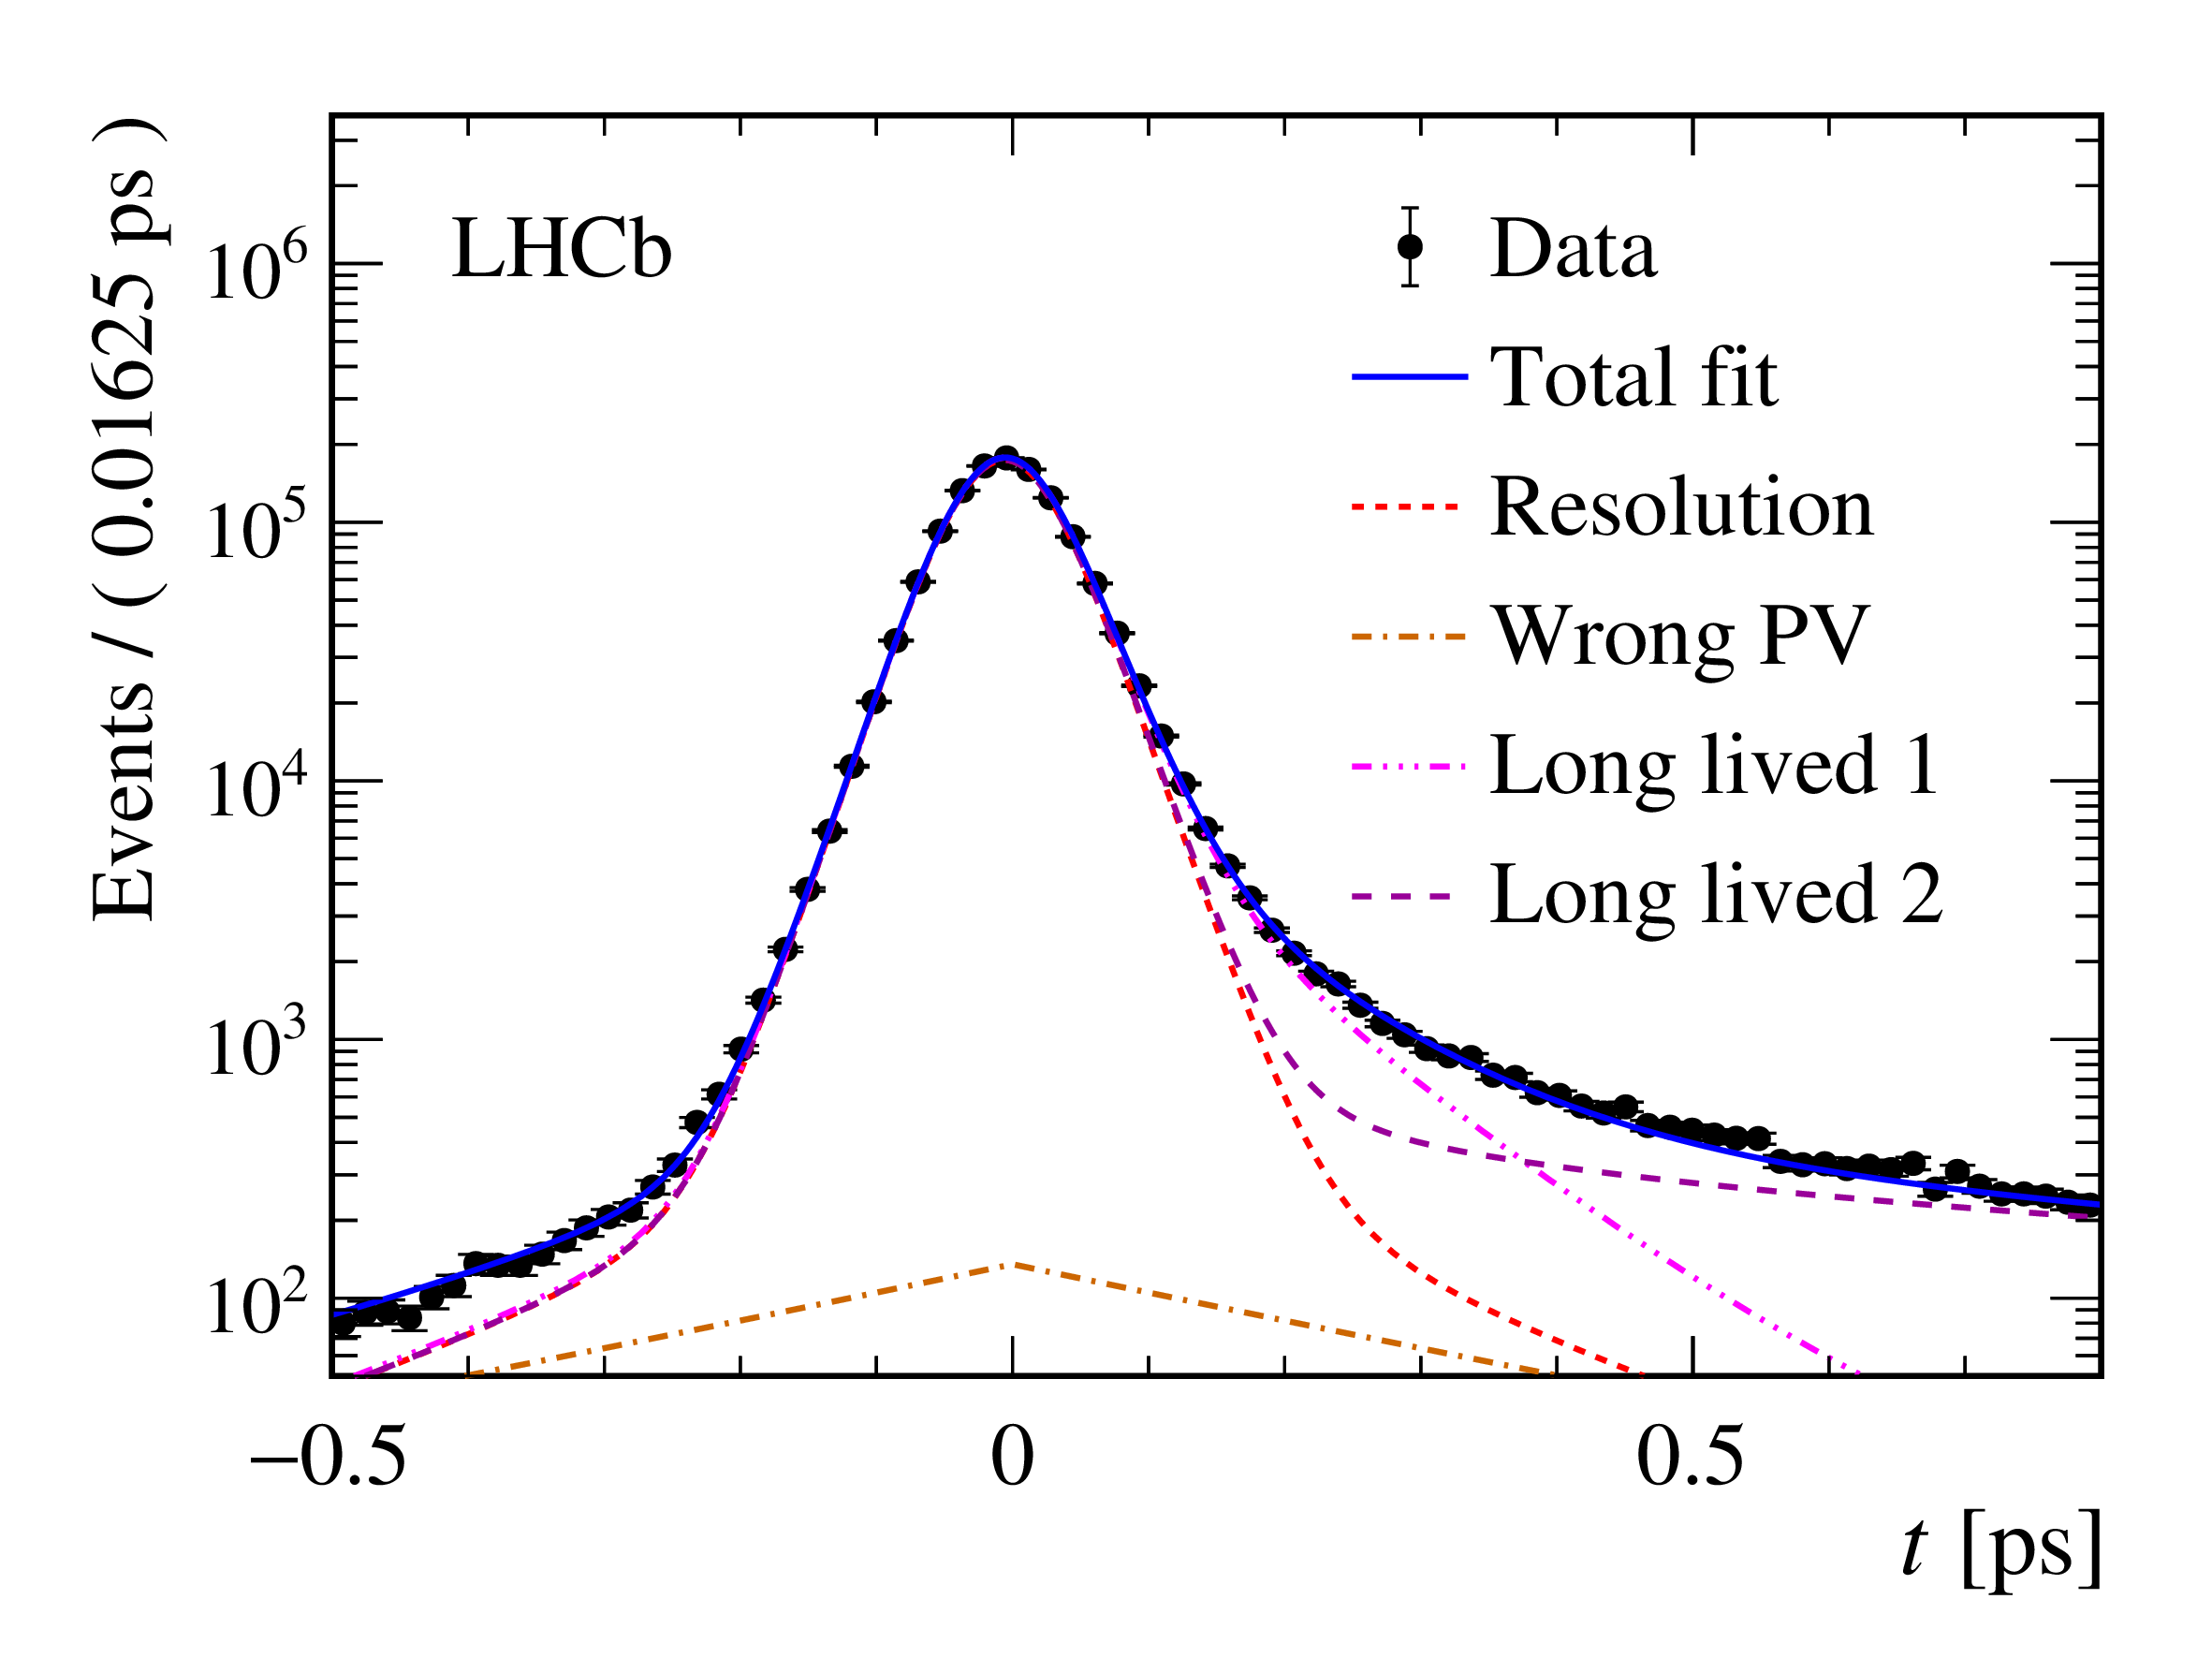
\includegraphics[width=\textwidth]{gpx/JpsiKK_time_res.png}
\end{column}

\begin{column}{0.45\textwidth}
$$ \sigma_{\text{eff}} = \sqrt{ \frac{-2}{\Delta m_s^2} 
\text{log} 
\left(\sum_{i=1}^3 f_i e^{-\sigma_i^2 \frac{\Delta m_s^2}{2}} \right) }$$

\medskip

  \begin{variableblock}{$B_s^0 \rightarrow J/\psi K^+
  K^-$}{bg=amber!20}{bg=amber}
  $$\sigma_{eff} \approx 45.5 \, \mathrm{fs}$$
  \end{variableblock}

  \begin{variableblock}{$B_s^0 \rightarrow J/\psi \pi^+
  \pi^-$}{bg=silver!20}{bg=silver}
  $$\sigma_{eff} \approx 41.5 \, \mathrm{fs}$$
  \end{variableblock}
\end{column}
\end{columns}

\pdfnote{Decay time in LHCb is computed as the flight distance of the B, from PV
to SV time ist mass divided by its momentum.}
\pdfnote{Resolution is obtained from a fit to promt sample formed form Jpsi and
to kaons from PV. Thus tau-prompt is zero.}
\pdfnote{The calibration is doen in bins of the per event decay time error from
vertex fit. It is modelled with 3 gaussian as we see from the formule}
\pdfnote{The effective resolution is 45.5 fs fro the KK mode and 41.5 fot PiPi}
\end{frame}
% }}}



\subsection{Decay-time efficiency} % {{{

\begin{frame}[default]
\frametitle{noframetitle}

\begin{columns}[b]

\begin{column}{0.45\textwidth}
  Product of individual splines for data and
  simulation to correct residual differences between signal and control samples:
  $$ \epsilon_{\text{data}}^{B_s^0} = \epsilon_{\text{data}}^{B_d^0}
  \frac{\epsilon_{\text{MC}}^{B_s^0}}
  {\epsilon_{\text{MC}}^{B_d^0}}.
  $$
  \vspace*{1cm}
  \begin{variableblock}{$B_s^0 \rightarrow J/\psi K^+
  K^-$}{bg=amber!20}{bg=amber}
  \begin{itemize}
    \item Using $B_d^0 \rightarrow J/\psi K^{*0}$.
    \item $\epsilon_{\text{data}}^{B_s^0}$ function of $\Gamma_d$ giving access
    to $\Gamma_s -\Gamma_d$ in final fit. 
  \end{itemize}
  \end{variableblock}
\end{column}

\begin{column}{0.45\textwidth}
  \begin{center}
    \includegraphics[width=0.8\textwidth]{gpx/JpsiKK_time_acc_2016_unb.pdf}
  \end{center}

  \begin{variableblock}{$B_s^0 \rightarrow J/\psi \pi^+
  \pi^-$}{bg=silver!20}{bg=silver}
  \begin{itemize}
    \item Using $B_d^0 \rightarrow J/\psi K^{*0}$.
    \item $\epsilon_{\text{data}}^{B_s^0}$ function of $\Gamma_d$ giving access
    to $\Gamma_H -\Gamma_d$ in final fit. 
  \end{itemize}
  \end{variableblock}
\end{column}

\end{columns}

\pdfnote{}
\pdfnote{In time acceptance Bd2JpsiKstar is used as control channel since it 
has a DG=0, hence the time dependent part factorices from the angular one. 
To do so we use 3 splines that model the decay time acceptance. 
Each of the splies models the efficiency from a different dataset BsMC, 
BdMC and BdData. These 3 splines are combined as in the expression to finally
get the efficiency in Bs data}
\pdfnote{The splines are multipliying a exponential convoluted with a gaussian
of meand 0 and sigma equal to the resolution}
\pdfnote{Though Bd and Bs decays are kinematically similar, we correct 
differences via some reweightings, between the samples in kinematics}
\end{frame}
% }}}



\subsection{Angular efficiency} % {{{

\begin{frame}[default]
\frametitle{noframetitle}

\begin{itemize}
  \item Selection and detector acceptance introduce efficiency effects in
  angular distributions.
  \begin{itemize}
    \item Also in $m(\pi\pi)$ in $B_s^0 \rightarrow J/\psi \pi^+ \pi^-$.
  \end{itemize}
  \item Efficiencies obtained from simulation iteratively corrected to match the
  data.
  \begin{itemize}
    \item $B_s^0 \rightarrow J/\psi K^+K^-$ validated with $B_d^0 \rightarrow
    J/\psi K^{*0}$.
  \end{itemize}
\end{itemize}

\begin{center}
  \begin{tabular}{cc}
    \includegraphics[width=0.25\textwidth]{gpx/BsJpsipipi_eff_chi.pdf}&
    \includegraphics[width=0.25\textwidth]{gpx/BsJpsipipi_eff_mpipi.pdf}\\
    \includegraphics[width=0.25\textwidth]{gpx/BsJpsipipi_eff_thetamu.pdf}&
    \includegraphics[width=0.25\textwidth]{gpx/BsJpsipipi_eff_thetapipi.pdf}
  \end{tabular}
\end{center}

\pdfnote{Selection and the intrinsic detector acceptance introduce efficiency
efectects in angular distributions. Also in the PiPi mass in BsJpsipipi, which
they have to correct too}
\pdfnote{We can divide it in to parts: the setup and the iterative procedure.}
\pdfnote{First a very naive set of angular acceptance weights is computed}
\pdfnote{Then we start a iterative procedure where MC is weighted to match data
in kinematics.}
\end{frame}
% }}}



\subsection{Flavor tagging} % {{{

\begin{frame}[default]
\frametitle{noframetitle}

Tagging in Run 2 improvement lead to 30 \% higher tagging power than Run 1:
\begin{itemize}
  \item $\epsilon (B_s^0\rightarrow J/\psi K^+K^-) = 4.73 \pm 0.34 \% $ (vs.
  $3.73\,\%$ in Run 1).  
  \item $\epsilon (B_s^0\rightarrow J/\psi \pi^+\pi^-) = 5.06 \pm 0.38 \% $ (vs.
  $3.89\,\%$ in Run 1).
\end{itemize}

\begin{center}
  \includegraphics[scale=0.6]{gpx/LHCb_tagging.pdf}
\end{center}

\pdfnote{Tagging is crucial for the phis measurement. Tagging was improved
between Run 1 and Run2 in about 30 per cent}
\pdfnote{We use both same side and opposite side kaon taggers.}
\end{frame}
% }}}



\subsection{Systematic uncertainties} % {{{

\begin{frame}
\frametitle{noframetitle}
\begin{columns}

\begin{column}{0.45\textwidth}
  \begin{variableblock}{$B_s^0 \rightarrow J/\psi K^+K^-$}
  {bg=amber!20}{bg=amber}
  \begin{itemize}
    \item Main syst. on $\phi_s$ is flavor tagging $\sim 0.015$ rad.
    \item Main syst. in $\Delta \Gamma$ comes from mass, angles and decay-time
    dependence, $\sim 0.0022\,\mathrm{ps^{-1}}$.
    \item Main syst. in $\Gamma_s - \Gamma_d$ comes from decay-time efficiency
    determination, $\sim 0.0012\,\mathrm{ps^{-1}}$.
    \item Main syst. in $\lambda$ comes from angular efficiency
    determination, $\sim 0.0043$.
  \end{itemize}
  \end{variableblock}
\end{column}

\begin{column}{0.45\textwidth}
  \begin{variableblock}{$B_s^0 \rightarrow J/\psi \pi^+\pi^-$}
  {bg=silver!20}{bg=silver}
  \begin{itemize}
    \item Main syst. on $\phi_s$ is the resonance modelling $\sim 9$ mrad.
    \item Main syst. in $\Gamma_H - \Gamma$ comes from background subtraction, 
    $\sim 3\,\mathrm{fs^{-1}}$.
    \item Main syst. in $\lambda$ is the resonance modelling, $\sim 0.0029$.
  \end{itemize}
  \end{variableblock}
\end{column}

\end{columns}

\pdfnote{Concerning sistematics in the main parameters.}
\pdfnote{Bs2JpsiKK phis main syst is indeed flavor tagging, while on BsJpsipipi
is the PiPi-resonace modelling.}
\pdfnote{The main syst in Gamma us the decay time efficiency in KK mode, but in
PiPi is the background subtraction.}
\pdfnote{The main syst in lambda comb from angular efficiency in KK, and again
because of resonace modelling in PiPi}
\pdfnote{Last, for DG in KK the main syst uncertainty comes from the mass,
angles and decay-time dependence}
\end{frame}
% }}}



\section{Current status}



\subsection{LHC$b$ combination} %{{{

\begin{frame}
  \frametitle{noframetitle}  
\vspace*{-5mm}
\begin{columns}
\begin{column}{0.45\textwidth}
  \begin{variableblock}{$B_s^0 \rightarrow J/\psi K^+K^-$}
  {bg=amber!20}{bg=amber}
  \vspace*{-3mm}
  \begin{align*}
    \phi_s & = -83 \pm 41 \pm 6 \, \mathrm{mrad} \\
    | \lambda | & = 1.012 \pm 0.016 \pm 0.006\\
    \Gamma_s - \Gamma_d & = -0.0041 \pm 0.0024 \pm 0.0015 \, \mathrm{ps^{-1}}\\
    \Delta \Gamma_s & = 0.077 \pm 0.008 \pm 0.003 \, \mathrm{ps^{-1}}
  \end{align*}
  \end{variableblock}
% \end{column}
%
% \begin{column}{0.45\textwidth}
  \begin{variableblock}{$B_s^0 \rightarrow J/\psi \pi^+\pi^-$}
  {bg=silver!20}{bg=silver}
  \vspace*{-3mm}
  \begin{align*}
    \phi_s & = -57 \pm 60 \pm 11 \, \mathrm{mrad} \\
    | \lambda | & = 1.01 {}_{-0.06}^{+0.08} \pm 0.03\\
    \Gamma_H - \Gamma_d & = -0.050 \pm 0.004 \pm 0.004 \, \mathrm{ps^{-1}}\\
  \end{align*}
  \end{variableblock}
\end{column}
\begin{column}{0.45\textwidth}
  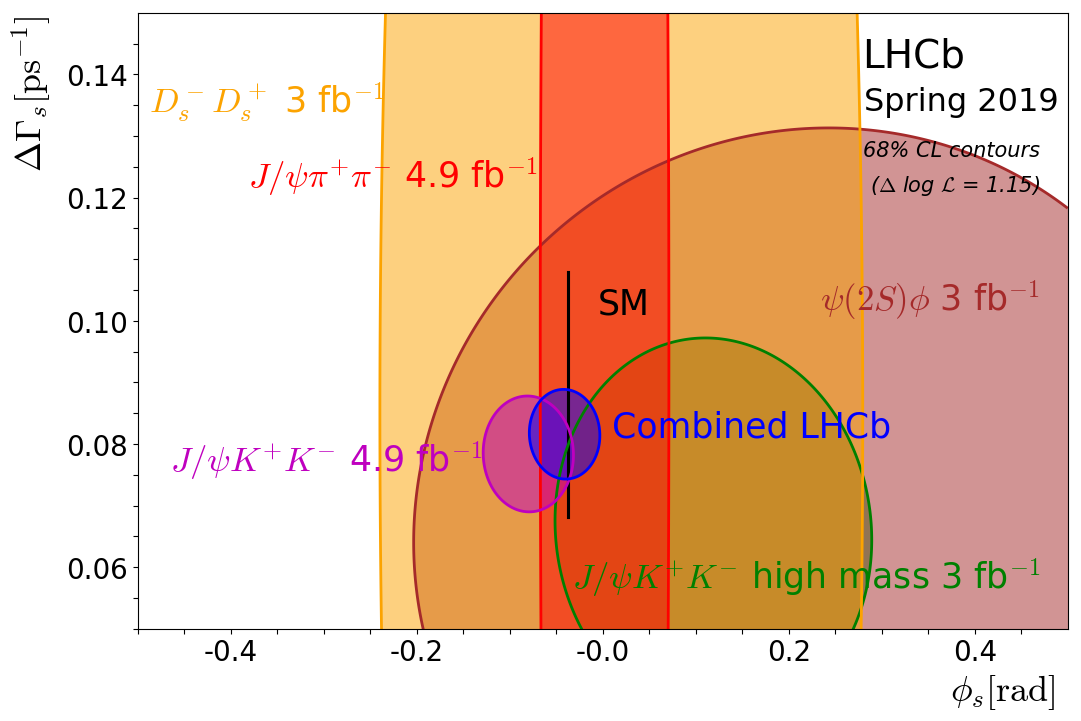
\includegraphics[width=\textwidth]{gpx/LHCb_Comb.png}
  
  \footnotesize
  \textbf{Run 1 :} 
  $B_s^0 \rightarrow D_s^- D_s^+$, [PRL 113 (2014) 211801] \\
  $B_s^0 \rightarrow J/\psi K^+ K^-$ (high mass) [JHEP 08 (2017) 037] \\
  and $B_s^0 \rightarrow \psi(2S) \phi$ [PLB 762 (2016) 253].

  \textbf{Run 1 + 15 + 16:}
  $B_s^0 \rightarrow J/\psi K^+ K^-$  [EPJC (2019) 79706] and \\
  $B_s^0 \rightarrow J/\psi \pi^+ \pi^-$ [PLB 797 (2019) 134789].
\end{column}
\end{columns}

\pdfnote{LHCb contributes to de WA with different measurements of phis. The main
ones as said, are BsJpsipipi and Bs2JpsiKK in the Phi region. These two channels
were analysed with 15 and 16 data too. But in Run1 alseo Bs2DsDs was analysed,
Bs2JpsiKK in the high mass region and Bs2Psi(2S)Phi.}
\pdfnote{At left we see the latest results from 2019 of Bs2JpsiKK and BsJpsipipi}
\pdfnote{17 and 18 data is currently being analysed}
\end{frame}



\subsection{HFLAV combination} % {{{

\begin{frame}[default]
\frametitle{noframetitle}

\begin{columns}[t]

  \begin{column}{0.55\textwidth}
    
    \vspace*{-0.6cm}
    \begin{columns}[t]

      \begin{column}{0.475\textwidth}
        \begin{variableblock}{$\phi_s$ \href{http://ckmfitter.in2p3.fr}
          {{CKMfitter}} (SM)}{bg=scqorange!20}{bg=scqorange}
         \centering  $\phi_s = -0.03696_{-0.00072}^{+0.00084}$ rad
        \end{variableblock}
        \begin{variableblock}{\href{https://arxiv.org/pdf/1511.09466.pdf}
          {{SM prediction}}}{bg=scqorange!20}{bg=scqorange}
         \centering  $\Delta \Gamma_s =  0.088 \pm 0.020\, \mathsf{ps}^{-1}$
         \centering  $\Gamma_s {}^{\dagger} = 0.6587 \pm 0.0024 \, \mathsf{ps}^{-1}$ 
        \end{variableblock}

        \begin{variableblock}{\href{https://arxiv.org/pdf/1511.09466.pdf}
          {{HFLAV}}}{bg=gray!20}{bg=gray}
         \centering  $\phi_s = -0.050 \pm 0.019$ rad
         \centering  $\Delta \Gamma_s =  0.0756 \pm 0.0059\, \mathsf{ps}^{-1}$
         \centering  $\Gamma_s = 0.6628 \pm 0.0035 \, \mathsf{ps}^{-1}$ 
        \end{variableblock}

        \tiny
        \rule{3cm}{0.1mm} \\
        \dagger: \\ Theory predicts
        $\frac{\Gamma_s}{\Gamma_d} = 1.0006\pm0.0025$. $\Gamma_s$
        is computed using the current WA $\Gamma_d = 1.519\pm 0.004$

      \end{column}



      \begin{column}{0.475\textwidth}

        \small 
        \begin{variableblock}{\href{https://cds.cern.ch/record/2668482/files/ATLAS-CONF-2019-009.pdf}
          {{ATLAS}} $99.7\,\mathrm{fb^{-1}}$}{bg=scqblue!20}{bg=scqblue}
          \centering $\phi_s = -0.076 \pm 0.034 \pm 0.019$ rad
          \centering $\Delta \Gamma = 0.068 \pm 0.004 \pm 0.003 \, \mathsf{ps}^{-1}$ 
          \centering $\Gamma_s = 0.669 \pm 0.001 \pm 0.001 \, \mathsf{ps}^{-1}$ 
        \end{variableblock}

        \small 
        \begin{variableblock}{\href{http://cds.cern.ch/record/2722794/files/BPH-20-001-arXiv.pdf}
          {{CMS}} $116\,\mathrm{fb^{-1}}$}{bg=scqred!20}{bg=scqred}
          \centering $\phi_s = -0.021 \pm 0.045$ rad 
          \centering $\Delta \Gamma = 0.1073 \pm 0.0097 \, \mathsf{ps}^{-1}$  
          \centering $\Gamma_s\!=\!0.6531\!\pm\!0.0042\!\pm\!0.0024\, \mathsf{ps}^{-1}$  
        \end{variableblock}
        
        \normalsize
        \begin{variableblock}{\href{https://arxiv.org/abs/1906.08356}
          {{LHC$b$}} $4.9\,\mathrm{fb^{-1}}$}{bg=scqgreen!20}{bg=scqgreen}
          \centering $\phi_s = -0.041 \pm 0.025$ rad 
          \centering $\Delta \Gamma = 0.0816 \pm 0.0048 \, \mathsf{ps}^{-1}$  
          \centering $\Gamma_s = 0.6562 \pm 0.0021 \, \mathsf{ps}^{-1}$  
        \end{variableblock}
        \tiny LHC$b$ includes more modes

      \end{column}

    \end{columns}



  \end{column}
  
  \begin{column}{0.3\paperwidth}
    \begin{center}
    \includegraphics[width=\textwidth]{gpx/PDG2021_Gs_vs_DGs.pdf}\\
    \vspace*{4mm}
    \includegraphics[width=\textwidth]{gpx/PDG2021_Phis_vs_DGs.pdf}
    \end{center}
  \end{column}
\end{columns}

\pdfnote{The main goal is to meassure the ooscillation phase,
the so called phis which is well predicted to be -2 beta s in the SM}
\pdfnote{Besides that, Gs via Gs minus Gd, DGs and DMs are also
measured}
\pdfnote{The SM prediction are presented here in the orange boxes against the
current status of the WA, which is dominated bu LHCb measurements}
\pdfnote{Latest averages, from Spring 2021, are presented too, were ATLAS
data up to 17 is included, whore Run2 of CMS and 15+16 of LHCb.}
\pdfnote{There exists tension between the tree experiments in Gamma and Delta
Gamma. ATLAS and LHCb differ in more than 4 sigma in their value of Gamma. Thats
the reason why these confidence bands are scaled}
\pdfnote{Results are consistent with SM-based global fits to data. There is
plenty of roo for New Phisics.}
\end{frame}
% }}}



\section{Prospects} % {{{

\begin{frame}
  \frametitle{nosubsection}

    \begin{itemize}
    \item ATLAS to analyse remaining Run 2 data from 2018, $\sim 40\,
    \mathrm{fb^{1}}$.
    \item CMS to add triggers and taggers to their full Run 2 dataset.
    \item LHC$b$ to analyse remaining Run 2 data from 2017 and 2018, $\sim
    4\, \mathrm{fb^{-1}}$.
      \begin{itemize}
      \item $B_s^0 \rightarrow J/\psi K^+ K^-$ should get to 
      $\sigma(\phi_s) \approx 22$ mrad from Run 1 + Run 2 alone. %In WG review.
      %\item $B_s^0 \rightarrow J/\psi \pi^+ \pi^-$ full Run 2 analysis is
      ongoing.
      \end{itemize}
    \end{itemize}
  
  \includegraphics[width=\textwidth]{gpx/integrated_luminosity.pdf}
  With $300\,\mathrm{fb^{-1}}$ LHC$b$ measurements of $\phi_s$ will be
  statistically dominated. 
  \begin{itemize}
    \item $\sigma_{\text{stat.}} (\phi_s) \approx 4 \text{ mrad}$ with $B_s^0
    \rightarrow J/\psi K^+ K^-$ ($ \approx 3 \text{ mrad}$ all modes
    combined).
    \item Improvements in trigger for $B_s^0 \rightarrow D_s^+ D_s^-$
    and adding other modes, i.e: $B_s^0 \rightarrow J/\psi(e^+ e^-) K^+ K^-$
  \end{itemize}

\pdfnote{Soonish the tree experiments are updating their measuremts. ATLAS is
about to add 2018 data. CMS is going to add triggers and taggers to their full
Run2 dataset}
\pdfnote{LHCb is currently analysing Run1 and full Run2 in Bs2JpsiKK with
should...}
\pdfnote{In the more distant future, with 300 inverse femtobarn LHCb
measurement of phis will bet statistically dominated. reaching up to 3 mrad all
modes combined. During next Runs of LHCb improvements on trigger to DsDs will be
done. And new modes will contribute to the LHCb average}
\end{frame}
% }}}



% END {{{
\begin{frame}[plain,overlaytitlepage=0.9,backgroundpicture=gpx/aiandes.pdf]
  \begin{minipage}[b][\textheight][b]{5cm}
    \includegraphics[height=0.5cm]{logos/igfae_bw}\hspace{1mm}
    \includegraphics[height=0.5cm]{logos/usc_bw}\hspace{1mm}
    \includegraphics[height=0.5cm]{logos/xunta_bw}\hspace{1mm}\\[2mm]
    \includegraphics[height=0.5cm]{logos/maeztu_bw}\hspace{1mm}
    \includegraphics[height=0.5cm]{logos/lhcb_bw}\\[-1mm]
  \end{minipage}

\pdfnote{And that's all. Thanks a lot for your attention and stay tuned. 
Updates are coming soon}
\end{frame}
% }}}
\end{document}
